\documentclass{beamer}
\usetheme{metropolis} % Use metropolis theme

\renewcommand{\footnoterule}{%
  \hspace{10cm}
  \kern -3pt
  \hrule width \textwidth height 1pt
  \kern 2pt
}
\usepackage[utf8]{inputenc}
\usepackage[T1]{fontenc}
\usepackage[british]{babel}
\usepackage[autostyle, english = british]{csquotes}
\usepackage[%
  backend=biber,
  doi=false,
  url=false,
  isbn=false,
  eprint=false,
  style=authoryear,
  hyperref=true,
  maxnames=2,
  minnames=1,
  maxbibnames=99,
  firstinits,
  uniquename=init]{biblatex}
\addbibresource{../bibliography.bib}

\usepackage{caption}
\usepackage{xpatch}
\usepackage{bm}
\usepackage{amsmath}
\usepackage{mathtools} % for \mathclap
\usepackage{varioref}
\usepackage{siunitx}
\usepackage{hyperref}
\usepackage[noabbrev]{cleveref}
\newcommand{\creflastconjunction}{, and\nobreakspace} % use Oxford comma
\usepackage{todonotes}
\usepackage{phaistos}
\usepackage{multimedia}
\usepackage{tikz}
\usetikzlibrary{arrows, positioning, shapes.geometric}
\usetikzlibrary{calc}
\usepackage{pgfgantt}


\graphicspath{{../../figures/}}

\newcommand{\cn}{\textbf{TODO: Citation}}

\title{Data-Driven Models for Zebrafish Motion\\IDP kick-off}
\author{Lukas Krenz}
\date{January 12, 2018} 
\institute{TUM, Chair for Computer Aided Medical Procedures \textit{\&} Augmented Reality}

\begin{document}
\maketitle
\begin{frame}{Introduction}
Collaboration with Couzin Lab (Max Plank Institute for Ornithology/University of Constance)

Advisers: Dr.\ Jacob Davidson (Constance), Nicola Rieke (CAMP)

Supervisor: Prof.\ Dr.\ Nassir Navab

Idea:
\begin{itemize}
\item Compare three data-driven models for motion of juvenile zebrafish
\item Model should capture motion of fish observed in experiments with \textbf{real fish} (\alert{not tracking} an individual fish)
\end{itemize}

Example \textbf{use case}: controlling a fish in a virtual reality environment
\end{frame}

\begin{frame}{Real and Virtual Zebrafish}
\begin{columns}
   \begin{column}{0.5\textwidth}
     \begin{figure}[h]
       \centering
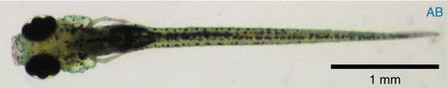
\includegraphics[clip, width=1\linewidth]{zebrafish.jpg}
       \caption*{A juvenile zebrafish}
     \end{figure}
   \end{column}
   
   \begin{column}{0.5\textwidth}
     \begin{figure}[h]
       \centering
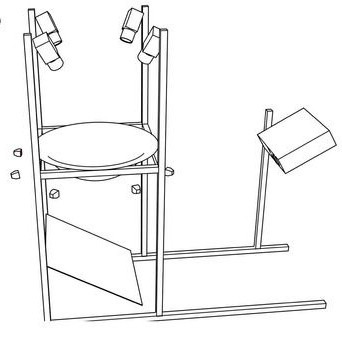
\includegraphics[clip, width=0.6\linewidth]{vr_zebrafish.jpg}
       \caption*{Virtual reality for zebrafish}
     \end{figure}
   \end{column}
\end{columns}
VR-paper and image source\footnote{\textit{Virtual reality for freely moving animals}, Nature Methods, 2017, Stowers JR, Hofbauer M, Bastien R, Griessner J, Higgins P, Farooqui S, Fischer RM, Nowikovsky K, Haubensak W, Couzin ID, Tessmar-Raible K. }
\end{frame}

\begin{frame}{Zebrafish: Burst-and-coast Motion} 
    \begin{figure}[H]
    \centering
    \movie[width=0.66\textwidth, height=0.66\textwidth, autostart,, loop, poster]{}{motion_experiment.mp4}
    \caption*{Example of zebrafish motion}
    \label{fig:calovi-sim}
  \end{figure}
\end{frame}

\begin{frame}
  \frametitle{Modelling Fish Motion}
Data: Roughly \textbf{100k kicks} from 10 experiments with 2 fish swimming, each for 1h

Videos already annotated, use trajectories (\alert{no tracking needed})

Segmentation into kicks as pre-processing step

Model \textbf{for each} fish: Map wall distance/angle and neighbour distance/angle to heading change $\delta \phi$
\begin{columns}
  \begin{column}{0.24\linewidth}
    \begin{figure}[h]
      \centering
    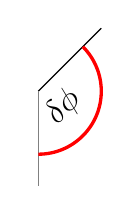
\begin{tikzpicture}[scale=0.4]
   \draw[] (3, 3)--(5,5); % our fish at t
   \node[rotate=45] at (4.5,4.5) {\textcolor{red}\PHtunny}; % head
   
   \draw[gray] (3.0, 0)--(3.0, 3.0); % fish at t - 1
   \node[rotate=90] at (3.0,2.5) {\textcolor{gray}\PHtunny}; % fish at t -1

   \draw [red,very thick] (3.0, 1.0) arc (-90:45:2);
   \node[rotate=45] at (3.8, 2.5) {\large$\delta\phi$};
 \end{tikzpicture} 
 \caption*{Heading change}
\end{figure}
\end{column}

\begin{column}{0.4\linewidth}
  \begin{figure}[h]
    \centering
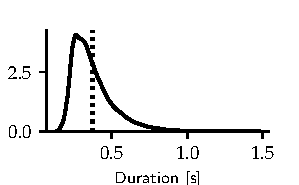
\includegraphics[clip, width=0.8\linewidth]{kick_duration.pdf}
    \caption*{Kick duration}
  \end{figure}
\end{column}

\begin{column}{0.4\linewidth}
  \begin{figure}[h]
    \centering
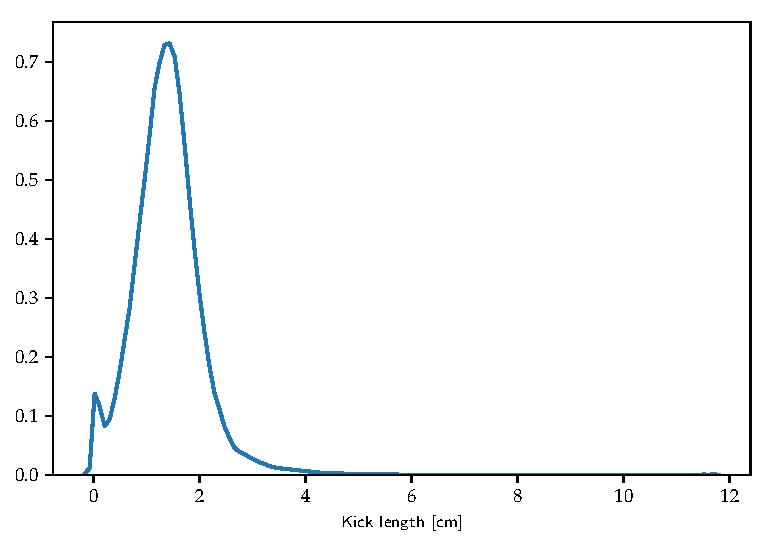
\includegraphics[clip, width=0.8\linewidth]{kick_length.pdf}
    \caption*{Kick length}
  \end{figure}
\end{column}

\end{columns}
\end{frame}

\begin{frame}{First Model: Force Based (Calovi et al\footnote{\hspace*{0.1cm}\textit{Disentangling and modeling interactions in fish with burst-and-coast swimming}, arXiv, 2017, Calovi, D.S., Litchinko, A., Lecheval, V., Lopez, U., Escudero, A.P., Chaté, H., Sire, C. and Theraulaz, G.})}
\begin{enumerate}
\item Discrete model, model heading change $\delta \phi$ for kicks
\item Decision process only uses \textbf{current status}
\item Force based, stochastic model
\item Symmetry constraints 
\end{enumerate}
Full model:
\begin{align*}
  \label{eq:calovi-model}
  \delta \phi &= \delta \phi_r (r_w) + \delta \phi_w (r_w, \theta_w) + \delta \phi_\text{Att} (d, \psi, \Delta \phi) + \delta \phi_\text{Ali}  (d, \psi, \Delta \phi) \\
  &= \text{noise} + \text{wall avoidance} + \text{attraction} + \text{alignment}
\end{align*}
with: $r_w$ distance to wall, $\theta_w$ angle towards wall,\\ $d$ distance between both fish, $\psi$ viewing angle and $\Delta \phi$ relative angle
\end{frame}

\begin{frame}
  \frametitle{Calovi - (Preliminary) Wall Fit}
 \begin{columns}
   \begin{column}{0.5\textwidth}
     \begin{figure}[h]
       \centering
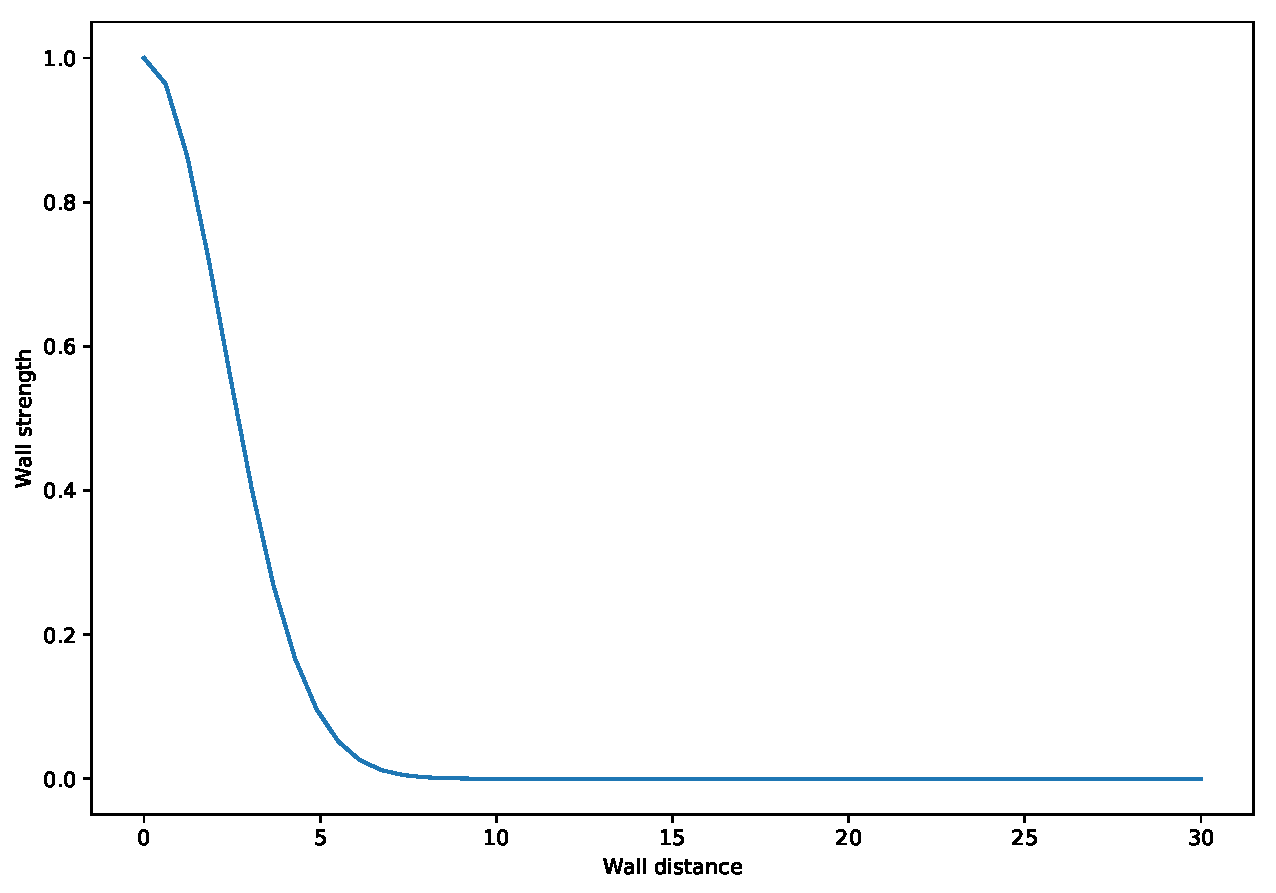
\includegraphics[clip, width=1\linewidth]{wall_force.pdf}
       \caption*{$f(r_w)$}
     \end{figure}
   \end{column}
   
   \begin{column}{0.5\textwidth}
     \begin{figure}[h]
       \centering
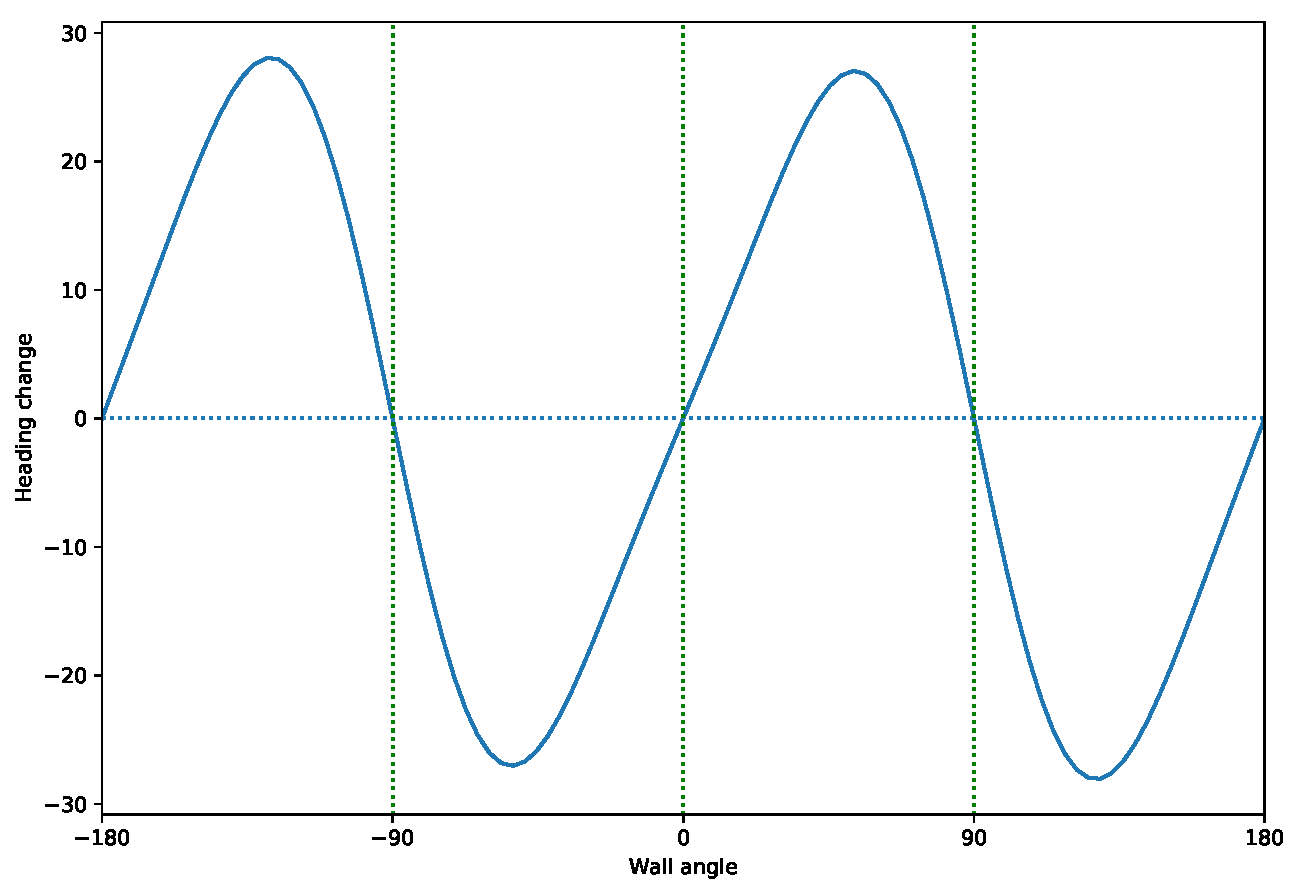
\includegraphics[clip, width=1\linewidth]{wall_odd.pdf}
       \caption*{$O(\theta_w)$}
     \end{figure}
   \end{column}
\end{columns}
\only<1>{
\begin{align*}
  \delta \phi_w (r_w, \theta_w) &= f(r_w)O_w(\theta_w) \\
  f(r_w) &= \exp\left( -{(r_w/l_w)}^2 \right) \\
  O(\theta_w) &= \left(a_1 \sin(\theta_w) + a_2 \sin(2  \theta_w)  \right)  \left(1 +  b_1  \cos(\theta_w) + b_2 \cos(2  \theta_w) \right)
\end{align*}
$r_w$ distance to wall, $\theta_w$ angle towards wall
}
\only<2>{
 \begin{columns}
   \centering
   \begin{column}{0.5\textwidth}
     \centering
  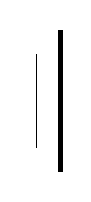
\begin{tikzpicture}[scale=0.3]
   \draw (3,-2)--(3,2); %fish
   \draw[ultra thick] (4,-3)--(4,3);
   \node[rotate=-90] at (3,-1) {\PHtunny};
 \end{tikzpicture}\qquad\qquad
  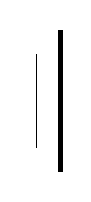
\begin{tikzpicture}[scale=0.3]
   \draw (3,-2)--(3,2); %fish
   \draw[ultra thick] (4,-3)--(4,3);
   \node[rotate=90] at (3,1) {\PHtunny};
 \end{tikzpicture}
 
\textbf{Stable fixed points}\\\ang{-90} and \ang{90}
   \end{column}
   \begin{column}{0.5\textwidth}
     \centering
  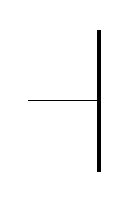
\begin{tikzpicture}[scale=0.3]
   \draw (0,0)--(3,0); % fish
   \draw[ultra thick] (3,-3)--(3,3);
   \node[rotate=180] at (1,0) {\PHtunny};
 \end{tikzpicture}\qquad\qquad
   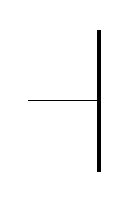
\begin{tikzpicture}[scale=0.3]
   \draw (0,0)--(3,0); % fish
   \draw[ultra thick] (3,-3)--(3,3);
   \node[rotate=0] at (2,0) {\PHtunny};
 \end{tikzpicture}

\textbf{Unstable fixed points}\\\ang{0}, \ang{-180} and \ang{180}  
   \end{column}
   
 \end{columns}
} 

\end{frame}

\begin{frame}
  \frametitle{Calovi - First simulation}
\begin{figure}[H]
    \centering
    \movie[width=0.66\textwidth, height=0.66\textwidth, autostart,, loop, poster]{}{wall_animation.mp4}
    \caption*{First simulation for wall model}
    \label{fig:calovi-sim}
\end{figure}
\end{frame}

\begin{frame}
  \frametitle{Second model: Spatio-Temporal Receptive Field}
 \begin{columns}
   \begin{column}{0.5\textwidth}
  \begin{tikzpicture}[scale=0.5]
   %\draw[red] (3, 3)--(5,5);
   \draw[ultra thick] (0,0)--(0,5);
   %\draw (4,-3)--(4,3);
   \node[rotate=45] at (4.5,4.5) {\textcolor{red}\PHtunny};
   \node[rotate=90] at (2.5,2.5) {\PHtunny};
   \node[rotate=90] at (2.5,0.5) {\textcolor{white}\PHtunny}; % quick hack to align stuff
 \end{tikzpicture}

 \textbf{No memory}: Only current position, etc.
\end{column}~\begin{column}{0.5\textwidth}
  \begin{tikzpicture}[scale=0.5]
   \draw[red] (3, 3)--(5,5); % our fish
   \draw[ultra thick] (0,0)--(0,5); % wall
   \draw[gray] (2.5, 0)--(2.5,2.5);
   \node[rotate=45] at (4.5,4.5) {\textcolor{red}\PHtunny};
   \node[rotate=90] at (2.5,2.5) {\PHtunny};
   \node[rotate=90] at (2.5,0.5) {\textcolor{gray}\PHtunny};
 \end{tikzpicture}

 \textbf{Memory}: Current position and trace
   \end{column}
 \end{columns}
  Drop assumption that kick is influenced only by current surroundings

  Inspired by computational neuroscience

  Approximate reaction to social forces by \textbf{weighted sum} over past environment influences (e.g.\ distances, angles)

  Linear model with memory
\end{frame}

\begin{frame}
  \frametitle{Third Model: Neural Network}
  Some evidence\footnote{\textit{Inferring the structure and dynamics of interactions in schooling fish}, Proceedings of the National Academy of Sciences, 2011, Katz, Y., Tunstrøm, K., Ioannou, C. C., Huepe, C., and Couzin, I. D.} for non-linear effects in collective animal motion

  Idea: Approximate reaction to social influences with a neural network

  Time series data, strong autocorrelation

  Use models such as \textbf{recurrent neural networks} (e.g.\ LSTM, GRU) or causal convolutional networks
  
  Highly non-linear model with memory
\end{frame}

\begin{frame}
  \frametitle{Summary and timeline}
\begin{itemize}
  \item Calovi: Linear model without memory
  \item Spatio-Temporal Receptive Field: Linear model with memory
  \item Neural Network: Non-linear model with memory 
\end{itemize}
  
 \begin{figure}[ftbp]
  \centering
  \begin{ganttchart}[
    time slot format=isodate,
    x unit=0.40mm,
    today=2018-01-12,
    y unit chart=5mm,
    ]{2017-10-01}{2018-04-30}
\gantttitlecalendar{year, month} \\
\ganttbar{Pre-processing}{2017-10-19}{2018-02-01}\\
\ganttgroup{Modelling}{2017-11-22}{2018-04-15}\\
\ganttbar{Calovi}{2017-11-22}{2018-02-01}\\
\ganttbar{Receptive Field}{2018-01-22}{2018-03-15}\\
\ganttbar{Neural Network}{2018-02-15}{2018-04-15}
\end{ganttchart}
\end{figure} 
\end{frame}

\section{Appendix}

\begin{frame}{Calovi - Only wall}
Consider no social component:
 \begin{equation*}
  \label{eq:calovi-wall_model}
  \delta \phi = \delta \phi_r (r_w) + \delta \phi_w (r_w, \theta_w)
\end{equation*}
Symmetry for wall influence:
\begin{equation*}
  \label{eq:calovi-wall-symmetry}
   \delta \phi_w (r_w, -\theta_w) =  - \delta \phi_w (r_w, \theta_w)
\end{equation*}
Split into force term $f(r_w)$ and odd function $O_r(\theta_w)$ 
\begin{equation*}
  \label{eq:calovi-wall-split}
  \delta \phi_w (r_w, \theta_w) = f(r_w)O_w(\theta_w)
\end{equation*}
\begin{align*}
  \label{eq:calovi-wall-force}
  f(r_w) &= \exp\left( -{(r_w/l_w)}^2 \right) \\
  O(\theta_w) &= \left(a_1 \sin(\theta_w) + a_2 \sin(2  \theta_w)  \right)  \left(1 +  b_1  \cos(\theta_w) + b_2 \cos(2  \theta_w) \right)
\end{align*}
\end{frame}

\end{document}